\chapter{Comparaison GCM - CCM - OCB}

Lors de nos recherches nous avons constaté que les algorithmes fournissant à la fois la confidentialité, l'authenticité et l'intégrité sont: GCM, CCM, OCB, CWC, EAX et APM.

Mais parmi eux seulement trois sortent du lot : GCM, OCB et CCM. C'est pourquoi nous avons décidé d'écarter les autres algorithmes et de seulement comparer ces trois.


\section{CCM}

Comme son nom le suggère le mode CCM combine le mode CTR et le mode CBC-MAC. Ces deux modes "primitifs" sont combinés pour authentifier les données puis les encrypter. CBC-MAC permet dans un premier temps d'obtenir un tag d'authentification du message clair. Puis le message et le tag sont chiffrés en utilisant le mode CTR.



Le vecteur d'initialisation (IV) doit être choisi avec précaution car il ne doit jamais être utilisé plus d'une fois par clef. En effet le mode CCM est un dérivé du mode CTR.



Une idée essentielle est que la même clé de cryptage peut être utilisée à la fois pour l'authentification et l'encryptage, à condition que les valeurs de comptage utilisées dans le cryptage ne rentrent pas en collision avec le vecteur d'initialisation (IV) utilisé pour l'authentification.


\begin{figure}[!h]
  \centering
  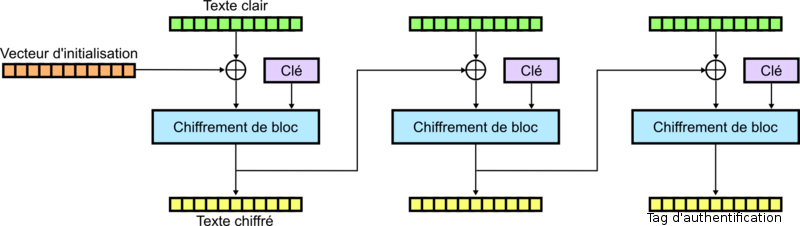
\includegraphics[width=\textwidth]{fonctionnement-CBC_MAC}
  \caption{Création du tag d'authentification avec CBC-MAC}
  \label{Création du tag d'authentification avec CBC-MAC}
\end{figure}

\begin{figure}[!h]
  \centering
  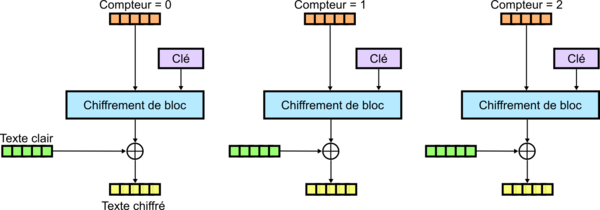
\includegraphics[width=\textwidth]{fonctionnement-CTR}
  \caption{Chiffrement du tag et du message avec CTR}
  \label{Chiffrement du tag et du message avec CTR}
\end{figure}


Contrairement à \aes, la génération du tag d'authentification (via CBC-MAC) est faite à partir du message en clair et non pas à partir du message encrypté. Au niveau performance, le mode CCM va utiliser de manière générale plus de calculs que \aes. En effet, dans \aes l'authentification et l'encryption ne font appel qu'une seule fois à l'algorithme AES par bloc, tandis que, le mode CCM va utiliser une première fois le chiffrement AES pour l'encryption puis une seconde fois pour générer le tag d'authentification. De plus, le mode CCM ne peut pas être parallélisé.


\newpage


\section{OCB}
Le mode OCB est lui aussi conçu pour fournir à la fois l'authentification et la confidentialité. OCB (Offset CodeBook) est basé sur le mode ECB avec l'utilisation d'un vecteur d'initialisation. Pour l'authentification il faut d'abord effectuer un checksum du message clair, ce checksum est ensuite encrypté comme un block du message clair. 

\begin{figure}[!h]
  \centering
  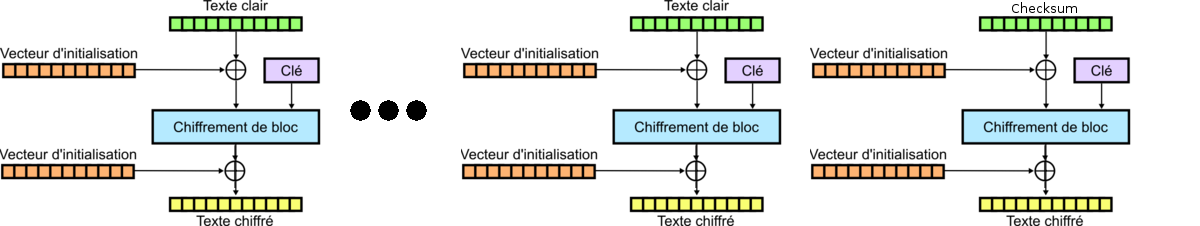
\includegraphics[width=\textwidth]{fonctionnement-OCB}
  \caption{Fonctionnement du mode OCB}
  \label{Fonctionnement du mode OCB}
\end{figure}

AES-OCB est un mode de fonctionnement qui est soumis à deux brevets aux Etat-Unis qui empêchent son utilisation dans toute application commerciale ou gouvernementale aux Etat-Unis. 
De plus Niels Ferguson a montré l'existence d'attaques sur le mode OCB qui limitent l'envoi de données à 64GB par clef. D'un point de vue performance, le mode OCB semble plus rapide que \aes car il ne nécessite pas l'implémentation des blocs de multiplications dans l'espace de Galois.


\section{Comparaison des performances}

\subsection{comparaison extrait d'une étude}


Pour obtenir les performances de ces modes nous nous sommes appuyés sur le travail de Ted KROVETZ et Phillip ROGAWAY \cite{compa}.

Sur la figure \ref{fig:compa}, il est possible d'observer la rapidité de modes OCB, CCM et GCM sur des architectures différentes. Sur l'axe des abscisses on peut observer la taille du message en bytes, et sur les ordonnées le nombre de cycles par byte.

On remarque que sur la totalité des architectures testées OCB est plus performant que ses rivales.

\begin{figure}[!h]
  \centering
  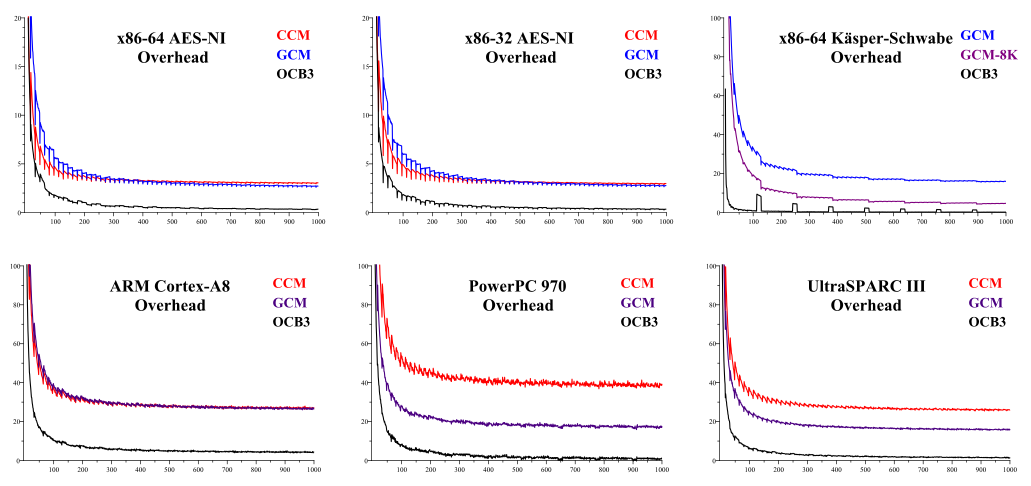
\includegraphics[width=\textwidth]{comparaison2}
  \caption{Performance empirique sur différents architectures\cite{compa}}
  \label{fig:compa}
\end{figure}

Cette étude confirme ce que nous avions révélé précédemment, \cad que OCB est plus performant que \aes.%Grâce à cette étude, nous pouvons en conclure que l'algorithme le plus performant est OCB en terme de rapidité. Ceci s'explique comme nous avons pu le remarquer précédemment sur la simplicité de l'algorithme.


\subsection{Comparaison réalisé sur nos machines personnelles}



Sur nos machines (Asus N76VB avec Ubuntu 14.04) nous avons également essayé de vérifier ces performances. Pour cela nous avons d'abord utilisé le site \url{http://www.faux-texte.com/lorem-ipsum-20.htm} pour générer un faux texte pseudo-aléatoire de 6.8M\footnote{Il est possible de visualiser le fichier que nous avons utilisé sur notre github \url{https://github.com/magichal/aes-gcm}} . Ensuite, nous avons exécuté la commande suivante dans notre terminal linux:

\begin{lstlisting}
  time openssl enc -e -in "fichier_test" -aes-256-gcm -out "fichier_encrypt" -k "toto"
\end{lstlisting}

  Voici la sortie que nous avons pu observer:

  \begin{lstlisting}
   openssl enc -e -in "fichier_test" -aes-256-gcm -out "fichier_encrypt" -k   0,02s user 0,01s system 98% cpu 0,027 total
  \end{lstlisting}

Donc notre ordinateur a mis 0.02s pour chiffrer notre fichier.

~\\

Malheureusement nous ne pourrons pas comparer cette performance aux mode OCB et CCM puisqu'ils ne sont pas implémentés dans openssl. Néanmoins, nous pouvons constater la rapidité de l'opération qui a été réalisée. Nous supposons que dans une utilisation courante cette rapidité est plus que suffisante pour un utilisateur lambda.

De plus au cours de notre réflexion nous avons envisagé de proposer une alternative à \aes en remplaçant AES par un autre algorithme de chiffrement. Nous pensons néanmoins que cela sort du cadre de notre étude c'est pourquoi il est possible de trouver en annexe à la page \pageref{anexe1} les alternatives à AES.




%%% Local Variables: 
%%% mode: latex
%%% TeX-master: "rapport_de_base"
%%% End: 
